\documentclass[10pt,twocolumn]{article}
\usepackage[margin=0.68in]{geometry}
\usepackage{amsmath,amssymb,amsthm}
\usepackage{graphicx}
\usepackage{booktabs}
\usepackage{multirow}
\usepackage{natbib}
\usepackage[hidelinks]{hyperref}
\newtheorem{theorem}{Theorem}
\newtheorem{lemma}[theorem]{Lemma}

\title{\textbf{DANG-Med: Dual-Stream Attention-Augmented Network with Prototype-Anchored Spatial Support and Gated Directional Strip Alignment for Multi-Center Polyp Segmentation}}

\author{
  OpenResearch Medical Vision Group \\
  \texttt{Department of Biomedical Engineering \& Computer Vision}
}
\date{\today}

\begin{document}
\maketitle

\begin{abstract}
Deep convolutional and vision transformer networks have achieved strong in-domain accuracy on curated colonoscopy benchmarks such as Kvasir-SEG ($\sim 93\%$ mDice), yet their segmentation reliability degrades under real-world clinical stress conditions: (i) severe label scarcity when adapting to new clinical centers ($5\%\text{--}10\%$ labeled frames), (ii) natural tiny ($<1.5\%$ mucosal area) and flat low-contrast camouflaged polyps across unseen imaging systems (e.g., ETIS-LaribPolypDB), and (iii) adverse endoscopic acquisition shifts including Narrow-Band Imaging (NBI) spectral emphasis, distal-lumen low-light falloff, and wet mucosal specular glare with motion defocus. To address these clinical failure modes on a single GPU, we propose \textbf{DANG-Med} (\textit{Dual-Stream Attention-Augmented Network with Prototype-Anchored Spatial Support and Gated Directional Strip Alignment}), a hybrid architecture coupling a local multi-scale ConvNeXt-Tiny hierarchy with a frozen DINOv2-Base foundation backbone ($86.58\text{M}$ frozen parameters) adapted via Frequency-Routed Mixture-of-Experts Convolutional LoRA (\textbf{Freq-MoE Conv-LoRA}). DANG-Med introduces four architectural pillars: (1) a \textbf{4-Scale Learned DPT Multi-Layer Reassembler} with a \textbf{Dual-Prototype and Image-Adaptive Self-Support Margin Head} that separates polyp versus mucosa token manifolds under $40$-image few-shot supervision; (2) a \textbf{Prototype-Anchored Spatial Support Envelope (PASSE)} that suppresses isolated far-field false-positive background specks while reinforcing detected lesion cores; (3) a \textbf{Multi-Scale Homomorphic Retinex Chromatic Stem} paired with a \textbf{DINOv2-Conditioned Low-Frequency Style Calibrator} (with feature-space MixStyle); and (4) an \textbf{Uncertainty-Guided Reverse-Attention Directional Strip Decoder} (\textbf{FastAxialStripSSM}) modulated by normalized Bernoulli boundary variance $4p(1-p)$. We evaluate two protocols across deduplicated in-domain, multi-center out-of-distribution (PolypGen 6-center Dev $n=258$ and Extended $n=974$, CVC-ClinicDB, CVC-ColonDB, CVC-300, ETIS-LaribPolypDB), and synthetic adverse stress cohorts: (A) our primary \textbf{Round~9/10 zero-shot stem protocol} ($5\%$ few-shot, $n=40$, 5 seeds 42--46), where all models share the same primary segmentation objective and no adverse synthetic corruptions are used during training (\texttt{aug\_prob=0.0}); and (B) our \textbf{Round~8 protocol} ($10\%$ few-shot, $n=80$, Seed~42), where \texttt{R8e} activates in-family online adverse synthesis (\texttt{aug\_prob=0.55}). Across all 5 paired seeds (Seeds 42--46) under the $5\%$ few-shot protocol, \textbf{DANG-Med v4.1 Flagship (\texttt{R9e+R10d/e})} improves over the single-stream ConvNeXt-Tiny+FPN baseline (\texttt{R9a+R10a}) from $44.74 \pm 3.79\%$ to \textbf{$51.05 \pm 1.71\%$ mDice ($+6.31$~pp paired mean, $p=0.014$; Seed~42: $+10.79$~pp)} and from $16.22 \pm 3.87\%$ to \textbf{$30.65 \pm 1.16\%$ Boundary F1 ($+14.44$~pp, $p=0.002$; Seed~42: $+22.68$~pp)} on few-shot tiny/camouflaged lesions ($S_1\times S_2$, $n=310$); from $45.59 \pm 4.02\%$ to \textbf{$55.82 \pm 1.17\%$ mDice ($+10.23$~pp, $p=0.005$)} on zero-shot adverse endoscopy ($S_1\times S_3$, $n=258$); and from $66.59 \pm 3.84\%$ to \textbf{$71.86 \pm 0.34\%$ mDice ($+5.27$~pp, $p=0.038$; Seed~42: $+11.86$~pp)} and $28.45 \pm 4.82\%$ to \textbf{$42.25 \pm 1.58\%$ BF1 ($+13.80$~pp)} on external PraNet benchmarks ($S_1\to\text{PraNet-Ext}$, $n=696$). Across all 5 paired seeds on full-data training ($n=800$), zero-shot \textbf{DANG-Med v4.1} reaches \textbf{$78.88 \pm 1.50\%$ mDice on ETIS-LaribPolypDB} (vs.\ $72.55 \pm 2.68\%$ baseline, $+6.33$~pp, $p=0.005$; Seed~42: $80.78\%$) and \textbf{$81.82 \pm 0.64\%$ on PraNet-Ext} (vs.\ $78.66 \pm 1.55\%$, $p=0.003$), while Round~8 \textbf{DANG-Med v4 (\texttt{R8e})} reaches \textbf{$81.53\%$ mDice on ETIS-LaribPolypDB} and \textbf{$73.87\%$ mDice on corruption-matched Adverse Endoscopy ($S_3$, $n=272$)}.
\end{abstract}

\section{Introduction}
Colorectal cancer (CRC) remains one of the leading causes of cancer-related mortality worldwide, and early endoscopic detection and resection of adenomatous and sessile serrated polyps during optical colonoscopy significantly reduces CRC incidence~\citep{jha2020kvasir,ali2023polypgen}. Automated pixel-level polyp segmentation provides computer-aided delineation (CADe/CADx) of lesion margins during withdrawal. However, a substantial gap persists between in-domain benchmark saturation and multi-center clinical deployment. On standard in-domain white-light colonoscopy splits such as Kvasir-SEG~\citep{jha2020kvasir}, modern hierarchical convolutional networks (e.g., ConvNeXt-Tiny~\citep{liu2022convnet} with Feature Pyramid Networks~\citep{lin2017fpn}) already achieve $92.5\%\text{--}93.1\%$ mean Dice (mDice). Under such saturated in-domain conditions, architectural modifications yield modest differences ($<0.5\text{--}1.0$~percentage points), obscuring whether a proposed model genuinely improves out-of-distribution (OOD) robustness.

In clinical practice, endoscopic segmentation systems degrade across three compounding stress axes:
\begin{enumerate}
  \item \textbf{Label-Scarce Multi-Center Adaptation ($S_1$):} Annotating pixel-accurate polyp contours requires expert gastroenterologists. When training under a strict $5\%\text{--}10\%$ annotation budget ($40\text{--}80$ labeled images), standard CNNs overfit to source-hospital background textures and suffer severe boundary degradation on external centers ($\text{Boundary F1} < 20\%$, $\text{HD95} > 70\,\text{px}$).
  \item \textbf{Natural Tiny and Low-Contrast Camouflaged Lesions ($S_2$):} Flat Paris~0-IIa/IIb adenomas and diminutive polyps occupying $<1.5\%$ of the endoscopic field of view (FOV) or exhibiting low RGB contrast ($<0.085$) against surrounding vascular mucosa are frequently missed or fragmented by stride-$16/32$ feature pooling, particularly on external cohorts such as ETIS-LaribPolypDB~\citep{silva2014toward} and CVC-ColonDB~\citep{tajbakhsh2015automated}.
  \item \textbf{Adverse Endoscopic Acquisition Shifts ($S_3$):} Endoscopic procedures frequently switch between White-Light Imaging (WLI) and Narrow-Band Imaging (NBI)-like spectral shifts, encounter distal-lumen illumination falloff ($\gamma > 2.2$ with sensor noise), and suffer from wet mucosal specular highlights coupled with motion/defocus blur.
\end{enumerate}

\begin{figure*}[t]
  \centering
  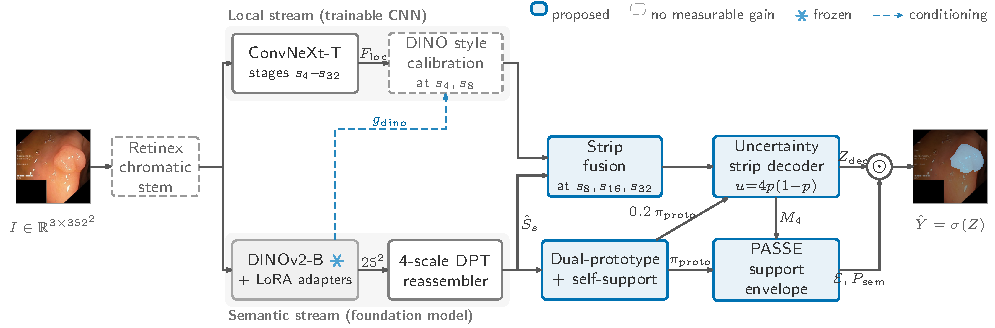
\includegraphics[width=\linewidth]{figs/arch_diagram.pdf}
  \caption{\textbf{Overview of the proposed DANG-Med architecture.} An input endoscopic frame ($352\times 352$) passes through the Multi-Scale Homomorphic Retinex Chromatic Stem (\texttt{RetinexChromaticStem}) to suppress specular highlights and standardize illumination/chrominance against source white-light EMA statistics. The local stream (ConvNeXt-Tiny stages $s_4..s_{32}$) captures sharp mucosal edges while the semantic stream (frozen DINOv2-Base with Freq-MoE Conv-LoRA on blocks $8..11$) extracts multi-depth $25\times 25$ patch tokens from layers $\{2,5,8,11\}$. Our highlighted contributions (blue) include DINO-Conditioned Low-Frequency Style Calibration, 4-Scale Learned DPT Reassembly, the Dual-Prototype \& Self-Support Margin Head, the Prototype-Anchored Spatial Support Envelope (PASSE), and the Uncertainty-Guided Reverse-Attention Directional Strip Decoder.}
  \label{fig:arch}
\end{figure*}

While Vision Foundation Models (VFMs) such as DINOv2~\citep{oquab2024dinov2} and SAM~\citep{kirillov2023segment} offer strong semantic invariance across domains, their coarse patch grids ($14\times 14$ stride) lack fine sub-pixel boundary localization. Conversely, naive feature concatenation between a CNN encoder and a ViT backbone can degrade high-resolution CNN edge features when ViT patch tokens are bilinearly upsampled across lesion boundaries, and sequential 2D state-space scans (SS2D~\citep{liu2024vmamba}) incur substantial Python/CUDA kernel launch overhead on multi-scale feature pyramids.

In this work, we present \textbf{DANG-Med}, illustrated in Figure~\ref{fig:arch}. Our main contributions are:
\begin{itemize}
  \item \textbf{Auditable Multi-Center Deduplication Hygiene and Clinical Stress Evaluation:} We implement an automated perceptual-hash and MD5 deduplication pipeline (\texttt{HYGIENE\_MANIFEST\_JSON}) across Kvasir-SEG, $6$-center PolypGen~\citep{ali2023polypgen} (Dev $n=258$ and untouched Extended Holdout $n=974$ in Round~9/10; $n=272$ and $n=967$ in Round~8), all $4$ official PraNet external benchmarks~\citep{fan2020pranet} ($n=696$ after removing $2$ exact/FOV duplicates against Kvasir: CVC-300 $n=60$, CVC-ClinicDB $n=61$, CVC-ColonDB $n=379$, ETIS-LaribPolypDB $n=196$), and derived stress slices ($S_1$ $5\%/10\%$ few-shot, $S_2$ pooled tiny/camouflaged lesions $n=310/315$, and $S_3$ synthetic adverse acquisitions $n=258/272$).
  \item \textbf{4-Scale DPT Reassembly, Dual-Prototype Self-Support, and PASSE Envelope:} We project multi-depth DINOv2 tokens into an $L_2$-normalized prototype hypersphere combining orthogonally initialized $K$-prototype cosine margins, training-gated ground-truth EMA support anchors, and test-time image-adaptive self-support centroids. Crucially, we introduce the \textbf{Prototype-Anchored Spatial Support Envelope (PASSE)}, which forms a dilated semantic support envelope to suppress far-field false-positive background specks on detected lesions while reinforcing low-contrast polyp cores.
  \item \textbf{Retinex Chromatic Stem and DINO-Conditioned Style Calibration:} We design a differentiable homomorphic Retinex stem (\texttt{RetinexChromaticStem}) paired with DINOv2-conditioned low-frequency style calibration and feature-space MixStyle at strides $4$ and $8$. We evaluate this module both under a strict zero-shot stem regime in Round~9/10 (\texttt{aug\_prob=0.0}, where the stem is performance-neutral relative to \texttt{ProtoDPT+PASSE} alone) and under corruption-matched online shift synthesis in Round~8 (\texttt{aug\_prob=0.55}).
  \item \textbf{Directional Strip Alignment and Uncertainty-Guided Reverse-Attention Decoder:} We formulate \textbf{FastAxialStripSSM} using fused cuDNN horizontal ($1\times 11, 7\times 1$), vertical ($11\times 1, 1\times 7$), and dilated ($3\times 3, d=3$) depthwise strip operators modulated by normalized Bernoulli boundary variance $u = 4p(1-p)$ and outer morphological ring halos.
\end{itemize}

\section{Related Work}
\subsection{Polyp Segmentation and Boundary-Aware Decoders}
Deep polyp segmentation architectures have progressed from U-Net~\citep{ronneberger2015unet} and UNet++~\citep{zhou2018unetplusplus} to reverse-attention and boundary-aware networks. PraNet~\citep{fan2020pranet} introduced parallel partial decoders and iterative reverse attention to mine boundary cues from Res2Net backbones. CaraNet~\citep{lou2022caranet} extended reverse attention with axial context and channel-wise feature pyramid modules for small medical objects. Subsequent Transformer-based architectures such as Polyp-PVT~\citep{dong2021polyp} and TransFuse~\citep{zhang2021transfuse} paired or replaced CNN encoders with Pyramid Vision Transformers to improve multi-center generalization on CVC-ColonDB and ETIS-LaribPolypDB. Unlike dual-branch models that fuse features only at coarse $1/16$ and $1/32$ scales with unconstrained bilinear upsampling, DANG-Med performs 4-scale learned DPT depth mixing with content-aware edge-snapped upsampling and explicit spatial support gating at stride~$4$ ($88\times 88$).

\subsection{Vision Foundation Models and Parameter-Efficient Adaptation}
Self-supervised Vision Transformers pretrained via discriminative self-distillation, notably DINOv2~\citep{oquab2024dinov2}, exhibit strong part-level semantic consistency across domains, while promptable foundation models such as SAM~\citep{kirillov2023segment} and its medical adaptations require either bounding-box prompts or heavy decoder fine-tuning. Adapting VFMs to autonomous dense medical segmentation while preventing overfitting on small clinical datasets ($N \le 800$) benefits from parameter-efficient fine-tuning (PEFT) such as LoRA~\citep{hu2022lora} and Dense Prediction Transformers (DPT)~\citep{ranftl2021vision}. We freeze $100\%$ of the DINOv2-Base backbone ($86.58\text{M}$ frozen parameters logged across all dual-stream runs) and inject lightweight Frequency-Routed Mixture-of-Experts Convolutional LoRA (\textbf{Freq-MoE Conv-LoRA}) adapters into blocks $8\text{--}11$, decomposing spatial tokens into low-frequency context and high-frequency edge energy routed across dilation rates $d \in \{1,2,3\}$.

\subsection{State-Space and Directional Strip Operators in Medical Vision}
Structured State-Space Sequence Models (S4, Mamba~\citep{gu2023mamba}) and 2D visual extensions (VMamba~\citep{liu2024vmamba}, U-Mamba~\citep{ma2024umamba}) model long-range spatial dependencies. However, executing recursive 4-directional 1D scans in Python across multi-scale 2D feature pyramids incurs substantial kernel launch overhead. Motivated by the connection between truncated state-space convolutional kernels and directional strip convolutions, our \textbf{FastAxialStripSSM} captures horizontal, vertical, and dilated contextual dependencies using fused depthwise strip convolutions gated by cross-stream conditioning, achieving $17.4\text{--}20.0$~FPS (measured at batch size $1$, $352\times 352$, FP16 on NVIDIA T4).

\section{Methodology: The DANG-Med Architecture}
Given an input endoscopic RGB image $I \in \mathbb{R}^{B \times 3 \times H \times W}$ ($H = W = 352$), DANG-Med (\texttt{src/dang/model.py}) predicts a dense foreground polyp probability map $\hat{Y} = \sigma(Z) \in [0, 1]^{B \times 1 \times H \times W}$. Figure~\ref{fig:arch} illustrates the complete pipeline.

\subsection{Retinex Chromatic Stem and DINO-Conditioned Style Calibrator}
Endoscopic frames from external centers or adverse modes exhibit non-uniform illumination and spectral shifts. Let $X_{\text{rgb}} \in [0, 1]^{B \times 3 \times H \times W}$ denote the unnormalized RGB image entering \texttt{RetinexChromaticStem} (instantiated in code whenever \texttt{use\_style\_calib=True}).
\paragraph{1) Specular Highlight Inpainting:} Mucosal glare saturates all three RGB channels. We detect specular pixels via a smooth minimum-channel gate $w_{\text{glare}} = \sigma(18.0 \cdot (\min_c X_{\text{rgb}} - 0.82))$ and blend them with a $15\times 15$ local average filter $\bar{X}_{15}$:
\begin{equation}
  X_{\text{deg}} = (1 - w_{\text{glare}}) X_{\text{rgb}} + w_{\text{glare}} \bar{X}_{15}.
  \label{eq:deglare}
\end{equation}
\paragraph{2) Multi-Scale Homomorphic Retinex Division:} Approximating image intensity as the product of illumination $L(x)$ and mucosal reflectance $R(x)$, we estimate illumination envelopes $L_{31} = \text{AvgPool}_{31\times 31}(X_{\text{deg}}) + \epsilon$ and $L_{15} = \text{AvgPool}_{15\times 15}(X_{\text{deg}}) + \epsilon$ ($\epsilon = 0.03$) and recover log-reflectance:
\begin{equation}
  \tilde{R} = \log(X_{\text{deg}} + \epsilon) - \bigl(0.65 \log L_{31} + 0.35 \log L_{15}\bigr).
  \label{eq:retinex}
\end{equation}
\paragraph{3) Source EMA Standardization and Anomaly Gate:} During training on source Kvasir-SEG images, the stem updates exponential moving average reference buffers $(\mu_{\text{ref}}, \sigma_{\text{ref}}) \in \mathbb{R}^{1\times 3\times 1\times 1}$ (in training mode only; frozen during \texttt{model.eval()}). In our Round~9/10 protocol (\texttt{R9d}, \texttt{R9e}, \texttt{R10d}, \texttt{R10e}), \texttt{aug\_prob} inside the stem is hard-set to $0.0$ so no synthetic adverse corruptions are generated during training (source-trained with mild photometric jitter $\gamma \in [0.8, 1.25]$, evaluated zero-shot on unseen $S_3$ synthetic corruptions where $\gamma = 2.55$). In Round~8 (\texttt{R8e}, commit \texttt{9539e96}), \texttt{aug\_prob=0.55} synthesizes NBI, low-light ($\gamma=2.35$), glare+blur, and combined corruptions with $0.55$ contrast compression during training; thus \texttt{R8e}'s $S_3$ score reflects in-family corruption-matched training rather than zero-shot OOD generalization. Combining instance-standardized reflectance $\hat{R}$ and global chromaticity $\hat{X}_{\text{deg}}$, the restored image is $X_{\text{rest}} = \text{clip}((0.55 \hat{X}_{\text{deg}} + 0.45 \hat{R}) \sigma_{\text{ref}} + \mu_{\text{ref}}, 0, 1)$. A photometric anomaly score $A_{\text{phot}}$ measures the normalized deviation of $( \mu(X_{\text{deg}}), \sigma(X_{\text{deg}}) )$ from $(\mu_{\text{ref}}, \sigma_{\text{ref}})$ plus glare fraction, gating a learned $3\times 3$ residual refinement branch (with minimum blend floor $0.04$).

At high-resolution ConvNeXt stages $s_4$ ($88\times 88$) and $s_8$ ($44\times 44$), \textbf{DINOFreqStyleCalibrator} first applies feature-space MixStyle~\citep{zhou2018unetplusplus} with probability $p=0.5$ ($\text{Beta}(0.1,0.1)$ instance-stat mixing across the batch during training only) and then decomposes local CNN features $F_{\text{loc}}$ into a $9\times 9$ low-frequency component $F_{\text{low}}$ and high-frequency detail $F_{\text{high}} = F_{\text{loc}} - F_{\text{low}}$, modulating both via affine parameters $(\gamma_{\text{low}}, \beta_{\text{low}}, \gamma_{\text{high}})$ predicted from the global DINOv2 context vector $g_{\text{dino}} \in \mathbb{R}^{B \times 768}$.

\subsection{4-Scale DPT Reassembly and Dual-Prototype Self-Support Margin Head}
We extract spatial token grids $\{T_\ell\}_{\ell \in \{2,5,8,11\}} \subset \mathbb{R}^{B \times 768 \times 25 \times 25}$ from DINOv2-Base (with Freq-MoE Conv-LoRA of rank $r=4$ on blocks $8\text{--}11$) and project each to $D = 192$ channels: $S_\ell = \text{ConvBNAct}_{1\times 1}(T_\ell)$.
\paragraph{4-Scale Learned DPT Reassembler:} We learn a $4\times 4$ depth-mixing matrix $W = \text{Softmax}(\Theta) \in \mathbb{R}^{4\times 4}$ across scales $s \in \{0,1,2,3\}$:
\begin{equation}
  \tilde{S}_s = \sum_{\ell=0}^{3} W_{s,\ell} S_\ell, \quad \hat{S}_s = \phi_s\bigl(\text{Up}_s(\tilde{S}_s, F_{\text{loc}}^{(s)})\bigr),
  \label{eq:dpt}
\end{equation}
where scales $s_8$ and $s_{16}$ use content-aware \textbf{Edge-Snapped Semantic Upsampling} (predicting $3\times 3$ local reassembly kernels from CNN features $F_{\text{loc}}^{(s)}$, initialized to bilinear interpolation).

\paragraph{Dual-Prototype and Self-Support Margin Head:} We concatenate $[S_1, S_2, S_3]$, project to $D_p = 128$ dimensions, and $L_2$-normalize across channels to obtain unit token embeddings $\hat{Z} \in \mathbb{R}^{B \times D_p \times 25 \times 25}$. We initialize $K=8$ learnable foreground prototypes $\{p_k^+\}_{k=1}^K$ and $K=8$ background prototypes $\{p_k^-\}_{k=1}^K$ orthogonally, alongside training-gated ground-truth EMA support anchors $(a^+, a^-)$ updated only during training from downsampled mask occupancy ($M_{25} \ge 0.35$ for foreground, $M_{25} \le 0.10$ for background). The prior cosine margin logit at each $25\times 25$ patch $(u,v)$ is:
\begin{align}
  \pi_{\text{prior}}(u,v) &= \tau \Bigl( \frac{1}{\beta}\log\sum_{k=1}^K e^{\beta \langle \hat{Z}_{u,v}, \hat{p}_k^+\rangle} - \frac{1}{\beta}\log\sum_{k=1}^K e^{\beta \langle \hat{Z}_{u,v}, \hat{p}_k^-\rangle} \Bigr) \nonumber \\
  &\quad + w_{\text{ema}} \cdot 10\bigl(\langle \hat{Z}_{u,v}, a^+\rangle - \langle \hat{Z}_{u,v}, a^-\rangle\bigr) + b.
  \label{eq:proto_prior}
\end{align}
During inference (without ground-truth masks), we compute image-specific self-support centroids $c^+ = \text{Norm}(\sum_{u,v} p_{u,v}^2 \hat{Z}_{u,v})$ and $c^- = \text{Norm}(\sum_{u,v} (1-p_{u,v})^2 \hat{Z}_{u,v})$ where $p_{u,v} = \sigma(\pi_{\text{prior}}(u,v))$, yielding the $25\times 25$ prototype margin map:
\begin{equation}
  \pi_{\text{proto}}(u,v) = \pi_{\text{prior}}(u,v) + 8w_{\text{ss}}\bigl(\langle \hat{Z}_{u,v}, c^+\rangle - \langle \hat{Z}_{u,v}, c^-\rangle\bigr).
  \label{eq:proto_total}
\end{equation}

\subsection{Prototype-Anchored Spatial Support Envelope (PASSE)}
While prototype priors strengthen semantic localization on detected lesions, uncalibrated high-frequency CNN texture noise far from the true polyp can cross the $0.5$ threshold, inflating false positives and $\text{HD95}$. To suppress far-field false positives without eroding lesion interiors, \textbf{PASSE} constructs a $25\times 25$ semantic probability map $P_{\text{sem}} = \sigma(0.5 M_4^{\uparrow 25} + 0.5 \pi_{\text{proto}})$ from the coarsest decoder stage logit $M_4$ and prototype logit $\pi_{\text{proto}}$ (falling back to $P_{\text{sem}} = \sigma(M_4^{\uparrow 25})$ when the prototype head is disabled, as in variant \texttt{R9d}), and computes a dilated smooth support envelope:
\begin{equation}
  \mathcal{E}_{\text{env}} = \text{AvgPool}_{3\times 3}\bigl(\text{MaxPool}_{5\times 5}(P_{\text{sem}})\bigr) \in [0,1]^{B\times 1\times 25\times 25}.
  \label{eq:passe_env}
\end{equation}
Upsampling $\mathcal{E}_{\text{env}}$ and $P_{\text{sem}}$ to stride~$4$ ($88\times 88$), PASSE modulates the stride-$4$ decoder logit $Z_{88}$ via two spatial terms, after which the final output logit blends the refined decoder prediction with the upsampled prototype margin when the prototype head is active:
\begin{align}
  Z_{88}^{\text{PASSE}} &= Z_{88} - 2.2\,\frac{\text{ReLU}(0.22 - \mathcal{E}_{\text{env}}^{\uparrow 88})}{0.22} + 1.2\,\text{ReLU}(P_{\text{sem}}^{\uparrow 88} - 0.38), \nonumber \\
  Z &= (1 - 0.2\,\mathbb{I}[\text{proto}])\bigl(Z_{88}^{\text{PASSE}}\bigr)^{\uparrow 352} + 0.2\,\mathbb{I}[\text{proto}]\,\pi_{\text{proto}}^{\uparrow 352}.
  \label{eq:passe_mod}
\end{align}

\subsection{Uncertainty-Guided Directional Strip Decoder}
At each pyramid scale $s \in \{s_8, s_{16}, s_{32}\}$, \textbf{GDSSAFusion} aligns local CNN features $F_{\text{loc}}^{(s)}$ and semantic features $\hat{S}_s$ using \textbf{FastAxialStripSSM}, a gated finite-kernel directional strip operator:
\begin{align}
  \text{StripSSM}(U, C) &= U + g_h \odot \mathcal{K}_{7\times 1}(\mathcal{K}_{1\times 11}(U)) \nonumber \\
  &\quad + g_v \odot \mathcal{K}_{1\times 7}(\mathcal{K}_{11\times 1}(U)) + g_d \odot \mathcal{K}_{3\times 3, d=3}(U),
  \label{eq:stripssm}
\end{align}
where $(g_h, g_v, g_d) = \sigma(\text{Conv}_{1\times 1}([U, C]))$ are input-conditioned directional gates and $\mathcal{K}$ denotes depthwise strip convolutions. In the top-down decoder ($P_4 \to P_3 \to P_2 \to P_1$), each \textbf{UncertaintyStripDecoderStage} computes from the coarser stage's logit $M_{s+1}^{\uparrow}$ three spatial priors: (i) foreground probability $A_{\text{fg}} = \sigma(M_{s+1}^{\uparrow})$, (ii) normalized Bernoulli boundary variance $U_s = 4 A_{\text{fg}}(1 - A_{\text{fg}}) \in [0,1]$ which peaks at $1.0$ along ambiguous borders ($A_{\text{fg}} = 0.5$), and (iii) an outer morphological ring halo $R_s = \text{clip}(\text{MaxPool}_{5\times 5}(A_{\text{fg}}) - A_{\text{fg}}, 0, 1)$, followed by A2BD Sobel-$L_1$ edge refinement.

\subsection{Training Objective and Variant Configuration Matrix}
In Round~9 and Round~10 (\texttt{R9a}--\texttt{R9e}, \texttt{R10a}--\texttt{R10e}), all arms use the exact same loss implementation \texttt{compute\_total\_loss} (\texttt{src/dang/train.py}, lines 103--140):
\begin{align}
  \mathcal{L}_{\text{total}} &= \mathcal{L}_{\text{BCE+Dice}}^{\tilde{w}}(Z, Y) + 0.25\,\mathcal{L}_{\text{Tversky}}^{\tilde{w},\alpha(a)}(Z, Y) + 0.10\,\mathcal{L}_{\text{far}}(Z, Y) \nonumber \\
  &\quad + 0.25\sum_{j=2}^4 \frac{1}{3}\mathcal{L}_{\text{BCE+Dice}}^{\tilde{w}}(M_j, Y) + 0.35\,\mathbb{I}[\text{proto}]\,\mathcal{L}_{\text{proto}}(\pi_{\text{proto}}, Y_{25}),
  \label{eq:loss}
\end{align}
where $a = 100 \cdot \bar{Y}$ is the ground-truth lesion area percentage, $w_i = \text{clip}((3.0 / (a_i + 0.35))^{0.40}, 1.0, 2.4)$ is normalized per batch via $\tilde{w}_i = w_i / \bar{w}$, $\alpha_{\text{fp}}(a) = 0.45 + 0.15\sigma((a - 1.5)/0.5)$ and $\beta_{\text{fn}}(a) = 1 - \alpha_{\text{fp}}(a)$ adapt Tversky supervision by lesion area, and $\mathcal{L}_{\text{far}}(Z, Y)$ averages $\sigma(Z_x)(1 - \text{Dilate}_r(Y)_x)$ across four dilation radii $r \in \{4,8,14,20\}\,\text{px}$ to penalize far-field false positives across all five arms. The auxiliary prototype supervision term $0.35\,\mathcal{L}_{\text{proto}}$ (applying $\mathcal{L}_{\text{BCE+Dice}}^{\tilde{w}} + 0.25\mathcal{L}_{\text{Tversky}}^{\tilde{w},\alpha(a)}$ to $\pi_{\text{proto}}$ vs.\ $Y_{25}$) is active whenever the architecture includes the prototype head ($\mathbb{I}[\text{proto}]=1$ in \texttt{R9c}, \texttt{R9e}, \texttt{R8c}, \texttt{R8e}; $\mathbb{I}[\text{proto}]=0$ in \texttt{R9a}, \texttt{R9b}, \texttt{R9d}, \texttt{R8a}, \texttt{R8b}, \texttt{R8d}). Specifically, the five Round~9 arms (differing only in \texttt{src/dang/config.py}) are configured as follows:
\begin{itemize}
  \item \textbf{\texttt{R9a} (Single-Stream Baseline, run \texttt{f328e771}, commit \texttt{e1379f6}):} ConvNeXt-Tiny + FPN decoder ($30.96\text{M}$ trainable / $30.96\text{M}$ total params), trained with Eq.~(\ref{eq:loss}) ($\mathbb{I}[\text{proto}]=0$).
  \item \textbf{\texttt{R9b} (Dual-Stream SafeConcat Control, run \texttt{e770b25c}, commit \texttt{946256c}):} ConvNeXt-Tiny + frozen DINOv2-Base ($86.58\text{M}$) with Freq-MoE Conv-LoRA + \texttt{fusion\_mode=safe\_concat} + FPN decoder ($33.57\text{M}$ trainable / $120.15\text{M}$ total params, $\mathbb{I}[\text{proto}]=0$).
  \item \textbf{\texttt{R9c} (DANG-v4.1 ProtoDPT + PASSE + UncStrip, No Stem, run \texttt{f676224f}, commit \texttt{1218ebb}):} Enables \texttt{use\_proto\_dpt=true}, \texttt{use\_passe\_envelope=true}, \texttt{fusion\_mode=proto\_dpt\_strip\_ssa}, \texttt{decoder\_mode=uncertainty\_strip\_ssm}, \texttt{use\_style\_calib=false} ($42.80\text{M}$ trainable / $129.38\text{M}$ total params, $\mathbb{I}[\text{proto}]=1$).
  \item \textbf{\texttt{R9d} (DANG-v4.1 RetinexStem + StyleCalib + PASSE + UncStrip, No ProtoDPT, run \texttt{5356b752}, commit \texttt{6d252bb}):} Enables \texttt{use\_style\_calib=true} (activating \texttt{RetinexChromaticStem} with zero-shot \texttt{aug\_prob=0.0} and MixStyle + \texttt{DINOFreqStyleCalibrator}), \texttt{use\_passe\_envelope=true}, \texttt{fusion\_mode=safe\_gd\_ssa\_v2}, \texttt{decoder\_mode=uncertainty\_strip\_ssm}, \texttt{use\_proto\_dpt=false} ($39.78\text{M}$ trainable / $126.36\text{M}$ total params, $\mathbb{I}[\text{proto}]=0$).
  \item \textbf{\texttt{R9e} (DANG-Med v4.1 Flagship, run \texttt{db1786be}, commit \texttt{a06b349}):} Enables all modules simultaneously: \texttt{use\_style\_calib=true} (\texttt{aug\_prob=0.0}), \texttt{use\_proto\_dpt=true}, \texttt{use\_passe\_envelope=true}, \texttt{fusion\_mode=proto\_dpt\_strip\_ssa}, \texttt{decoder\_mode=uncertainty\_strip\_ssm} ($43.32\text{M}$ trainable / $129.90\text{M}$ total params, $\mathbb{I}[\text{proto}]=1$).
\end{itemize}
In the earlier Round~8 exploration suite (\texttt{R8a} run \texttt{4ff780b9}, \texttt{R8b} run \texttt{eed6d338}, \texttt{R8c} run \texttt{02df9e4a}, \texttt{R8d} run \texttt{d47b9a4b}, \texttt{R8e} run \texttt{a8ecd157}), \texttt{R8a}--\texttt{R8d} used standard unweighted BCE+Dice+Tversky without $\mathcal{L}_{\text{far}}$ or PASSE (\texttt{R8c} used \texttt{decoder\_mode=detail\_a2bd\_v2} at $40.50\text{M}/127.08\text{M}$ params; \texttt{R8d} used \texttt{uncertainty\_strip\_ssm} without RetinexStem or adverse synthesis at $40.21\text{M}/126.79\text{M}$ params), whereas only \texttt{R8e} combined the scale-adaptive loss (without PASSE or $\mathcal{L}_{\text{far}}$) and online adverse stem corruption synthesis (\texttt{aug\_prob=0.55}). Because \texttt{R9} and \texttt{R8} differ across multiple factors simultaneously (loss formulation, PASSE, $5\%$ vs.\ $10\%$ $S_1$ budget, and $\text{dHash}_{64}\le 4$ tightening from $n=272\to 258$), Round~9/10 serves as our strictly controlled ablation suite while Round~8 is reported as a historical reference showing the upper bound when training corruptions match the $S_3$ test families.

\section{Experimental Setup and Data Hygiene}
\subsection{Datasets, Deduplication Hygiene, and Evaluation Cohorts}
Public composite polyp repositories (e.g., \texttt{combo\_polyp} / PolypGen) contain UUID-named Kvasir-SEG images in their raw splits and occasional near-duplicate frames. We enforce an automated deduplication pipeline (\texttt{src/dang/data.py}, logged via \texttt{HYGIENE\_MANIFEST\_JSON}):
\begin{enumerate}
  \item \textbf{In-Domain Kvasir-SEG ($n=1{,}000$ raw):} Shuffled (\texttt{seed=20260101}) into \textbf{Train-Full ($n=800$)}, \textbf{Train-$S_1$ Few-Shot ($5\%$, $n=40$ in R9/R10; $10\%$, $n=80$ in R8)}, \textbf{Val ($n=95$)}, and \textbf{ID-Test ($n=90$)}, where any validation or test image with $64$-bit perceptual difference hash distance $\text{dHash}_{64} \le 4$ to any training image is dropped ($5$ in Val, $10$ in ID-Test).
  \item \textbf{PolypGen 6-Center Out-of-Distribution (\texttt{C1}--\texttt{C6})~\citep{ali2023polypgen}:} Kvasir UUID filenames ($204$ in Dev, $796$ in Extended), empty masks ($30$ in Dev, $86$ in Extended), exact MD5 duplicates, and frames with $\min_{x \in \text{Kvasir}} \text{dHash}_{64} \le 4$ ($14$ in Dev, $78$ in Extended) are removed, yielding \textbf{PolypGen-Dev ($n=258$ in R9/R10; $n=272$ in R8 prior to the $\text{dHash}_{64}\le 4$ filter)} and \textbf{PolypGen-Extended Holdout ($n=974$ in R9/R10 after also filtering $47$ Dev near-duplicates and $49$ intra-Extended near-duplicates; $n=967$ in R8)}. We note that $74$ frames in PolypGen-Extended share \texttt{C4} video sequence prefixes with Dev; we therefore also track sequence-disjoint subsets in our logs.
  \item \textbf{PraNet Official External Benchmarks ($n=696$ total across 4 datasets)~\citep{fan2020pranet}:} After removing $2$ frames with exact/FOV-cropped $\text{dHash}_{64} \le 1$ overlap against Kvasir-SEG ($1$ in CVC-ClinicDB, $1$ in CVC-ColonDB), we evaluate: \textbf{CVC-300 ($n=60$)}, \textbf{CVC-ClinicDB ($n=61$)}, \textbf{CVC-ColonDB ($n=379$)}, and \textbf{ETIS-LaribPolypDB ($n=196$)}.
  \item \textbf{Derived Clinical Stress Track $S_2$ (Natural Tiny \& Camouflaged Polyps, $n=310$ in R9/R10; $n=315$ in R8):} Pooled across PolypGen-Dev, ETIS-LaribPolypDB, and CVC-ColonDB for natural lesions with area $<1.5\%$ of FOV (\texttt{S2\_Tiny\_LT1.5pct}, $n=188$) or area $<3.0\%$ with local boundary RGB contrast $<0.085$ (\texttt{S2\_Camouflaged\_LowContrast}, $n=122$). Because $S_2$ and $S_3$ are derived from the external cohorts above to isolate specific clinical failure modes, they are diagnostic stress slices rather than statistically independent patient cohorts.
  \item \textbf{Derived Clinical Stress Track $S_3$ (Synthetic Adverse Endoscopy, $n=258$ in R9/R10; $n=272$ in R8):} Deterministic transformations of PolypGen-Dev frames across $4$ regimes: \texttt{Adverse\_NBI\_Spectral}, \texttt{Adverse\_LowLight\_Lumen} ($\gamma=2.55$ + vignette + shot noise), \texttt{Adverse\_Specular\_Glare\_Blur}, and \texttt{Adverse\_Combined\_Severe}.
\end{enumerate}

\subsection{Implementation Details and Evaluation Metrics}
All models are trained at $352\times 352$ resolution ($350\times 350 = 25\times 25$ patches for DINOv2-Base) with batch size $16$, AdamW ($\text{lr}_{\text{cnn}} = 1.6\times 10^{-4}$, $\text{lr}_{\text{new}} = 4.0\times 10^{-4}$, $\text{lr}_{\text{peft}} = 1.0\times 10^{-3}$; weight decay $10^{-4}$ on CNN/head parameters and $0.0$ on PEFT/bias/normalization parameters), cosine annealing with warmup, EMA decay $0.992$, and FP16 mixed precision on NVIDIA T4 GPUs. Track~$S_1$ trains for $40$~epochs ($\sim 3.4\,\text{s/epoch}$ on \texttt{R9a}, $\sim 11.8\,\text{s/epoch}$ on \texttt{R9e}), and Track~Full trains for $20$~epochs ($\sim 20.4\,\text{s/epoch}$ on \texttt{R9a}, $\sim 72\text{--}80\,\text{s/epoch}$ on \texttt{R9e}). Checkpoint selection uses Kvasir-Val mDice exclusively (\texttt{model.eval()} never receives ground-truth masks).

At $352\times 352$ resolution with threshold $0.5$ (\texttt{src/dang/metrics.py}), we report \textbf{mDice ($\%$)}, \textbf{mIoU ($\%$)}, \textbf{Boundary F1 ($\%$)} ($1\text{-px}$ morphological contour with $2\text{-px}$ dilation tolerance), and \textbf{95th-percentile Hausdorff Distance ($\text{HD95}$, $\text{px}$)}. When a prediction mask is empty while the ground-truth mask is non-empty (or vice versa), $\text{BF1}=0$ and our implementation assigns a fixed finite quarter-diagonal penalty $\text{HD95}_{\text{empty}} = 0.25\sqrt{352^2+352^2} \approx 124.45\,\text{px}$; we also report non-empty-only Hausdorff distance (\texttt{hd95\_non\_empty}), empty-prediction miss rates (\texttt{ep}), and sensitivity across half-diagonal ($248.90\,\text{px}$) and full-diagonal ($497.80\,\text{px}$) penalties in Section~\ref{sec:multiseed}.

\begin{figure*}[t]
  \centering
  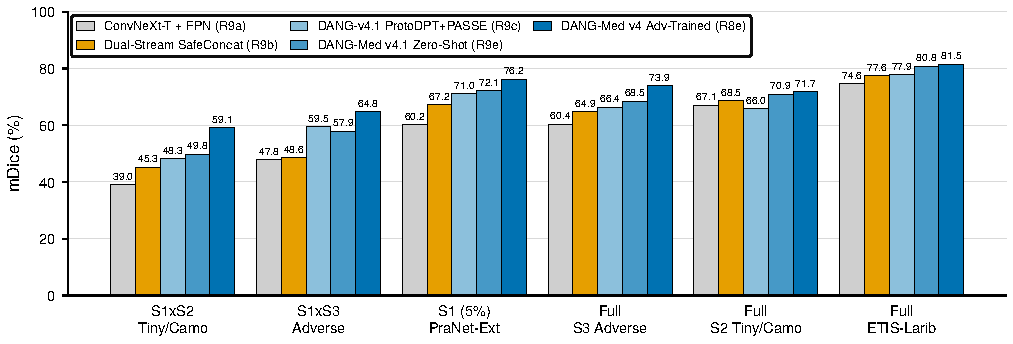
\includegraphics[width=\linewidth]{figs/stress_benchmarks.pdf}
  \caption{\textbf{Comparison of single-stream and dual-stream baselines against DANG-Med across six OOD and clinical stress benchmarks (Seed 42).} Mean Dice (mDice, $\%$) across few-shot tiny/camouflaged polyps ($S_1\times S_2$, $n=310/315$), few-shot adverse endoscopy ($S_1\times S_3$, $n=258/272$), few-shot external PraNet ($S_1$, $n=696$; $5\%$ labels in R9, $10\%$ in R8), full-data adverse endoscopy ($S_3$), full-data tiny/camouflaged polyps ($S_2$), and full-data ETIS-LaribPolypDB ($n=196$).}
  \label{fig:stress_bars}
\end{figure*}

\section{Experimental Results and Ablation Analysis}

\begin{table*}[t]
  \centering
  \caption{\textbf{Few-Shot Clinical Stress Benchmarks ($S_1$ Track, Seed 42): Round~9 Zero-Shot Stem Protocol (\texttt{R9a}--\texttt{R9e}, $5\%$ Kvasir labels, $n=40$) and Round~8 Protocol (\texttt{R8a}--\texttt{R8e}, $10\%$ Kvasir labels, $n=80$).} All values match raw \texttt{SEED\_SUMMARY\_JSON} logs to two decimal places. Cohort sizes in R9 (and R8 where different): $S_1\times S_2$ $n=310$ ($315$), $S_1\times S_3$ $n=258$ ($272$), $S_1\to\text{PraNet-Ext}$ $n=696$, and $S_1\to\text{PolypGen-Dev}$ $n=258$ ($272$). Gain rows ($\Delta$ and $\Delta\%$) are computed directly from unrounded log summaries. Note that in \texttt{R8e}, $S_3$ corruptions are matched to the online training synthesis (\texttt{aug\_prob=0.55}).}
  \label{tab:s1_stress}
  \vspace{2pt}
  \resizebox{\textwidth}{!}{%
  \begin{tabular}{l cccc cccc cccc cccc}
    \toprule
    \multirow{2}{*}{\textbf{Model Variant}} & \multicolumn{4}{c}{\textbf{$S_1 \times S_2$: Tiny/Camo ($n=310/315$)}} & \multicolumn{4}{c}{\textbf{$S_1 \times S_3$: Adverse ($n=258/272$)}} & \multicolumn{4}{c}{\textbf{$S_1 \to$ PraNet-Ext ($n=696$)}} & \multicolumn{4}{c}{\textbf{$S_1 \to$ PolypGen-Dev ($n=258/272$)}} \\
    \cmidrule(lr){2-5} \cmidrule(lr){6-9} \cmidrule(lr){10-13} \cmidrule(lr){14-17}
    & Dice$\uparrow$ & IoU$\uparrow$ & BF1$\uparrow$ & HD95$\downarrow$ & Dice$\uparrow$ & IoU$\uparrow$ & BF1$\uparrow$ & HD95$\downarrow$ & Dice$\uparrow$ & IoU$\uparrow$ & BF1$\uparrow$ & HD95$\downarrow$ & Dice$\uparrow$ & IoU$\uparrow$ & BF1$\uparrow$ & HD95$\downarrow$ \\
    \midrule
    \multicolumn{17}{l}{\textit{Round 9 Protocol ($5\%$ Few-Shot, $n=40$ Kvasir images; shared primary loss Eq.~(\ref{eq:loss}), zero-shot stem \texttt{aug\_prob=0}):}} \\
    \texttt{R9a}: ConvNeXt-T + FPN Baseline & 39.00 & 30.53 & 9.67 & 87.82 & 47.84 & 38.93 & 12.44 & 88.18 & 60.20 & 49.80 & 19.97 & 83.04 & 65.02 & 54.99 & 15.64 & 68.32 \\
    \texttt{R9b}: Dual-Stream SafeConcat + FPN & 45.26 & 37.50 & 17.45 & 71.04 & 48.55 & 40.28 & 15.97 & 85.08 & 67.20 & 58.33 & 29.47 & 60.37 & 67.50 & 58.61 & 25.24 & 59.72 \\
    \texttt{R9c}: DANG-v4.1 (ProtoDPT+PASSE+Unc) & 48.27 & 41.16 & 25.81 & 65.41 & \textbf{59.55} & \textbf{51.16} & 26.16 & \textbf{68.16} & 71.01 & 63.04 & 39.12 & 50.07 & 70.27 & 61.87 & 34.04 & 55.91 \\
    \texttt{R9d}: DANG-v4.1 (Retinex+Style+PASSE+Unc) & 45.99 & 39.55 & 25.53 & 66.31 & 53.43 & 45.75 & 25.35 & 80.38 & 68.69 & 61.46 & 39.30 & 48.20 & 69.49 & 60.94 & 34.27 & 55.90 \\
    \textbf{\texttt{R9e}: DANG-Med v4.1 Flagship} & \textbf{49.80} & \textbf{43.42} & \textbf{32.35} & \textbf{64.24} & 57.87 & 49.18 & \textbf{29.33} & 77.01 & \textbf{72.06} & \textbf{64.71} & \textbf{44.29} & \textbf{46.60} & \textbf{72.63} & \textbf{64.60} & \textbf{42.14} & \textbf{53.76} \\
    \midrule
    \textbf{Abs. Diff. (\texttt{R9e} vs. \texttt{R9a} Baseline)} & \textbf{+10.79} & \textbf{+12.88} & \textbf{+22.68} & \textbf{--23.58} & \textbf{+10.03} & \textbf{+10.25} & \textbf{+16.89} & \textbf{--11.18} & \textbf{+11.86} & \textbf{+14.90} & \textbf{+24.32} & \textbf{--36.44} & \textbf{+7.62} & \textbf{+9.61} & \textbf{+26.50} & \textbf{--14.56} \\
    \textit{Rel. Change $\Delta\%$ (\texttt{R9e} vs. \texttt{R9a})} & \textbf{+27.68\%} & \textbf{+42.20\%} & \textbf{+234.4\%} & \textbf{--26.85\%} & \textbf{+20.96\%} & \textbf{+26.32\%} & \textbf{+135.8\%} & --12.67\% & \textbf{+19.70\%} & \textbf{+29.93\%} & \textbf{+121.8\%} & \textbf{--43.88\%} & +11.72\% & \textbf{+17.48\%} & \textbf{+169.4\%} & \textbf{--21.31\%} \\
    \textbf{Abs. Diff. (\texttt{R9c} vs. \texttt{R9a} Baseline)} & +9.27 & +10.63 & +16.14 & --22.41 & \textbf{+11.70} & \textbf{+12.23} & +13.72 & \textbf{--20.02} & +10.81 & +13.23 & +19.14 & --32.97 & +5.25 & +6.88 & +18.40 & --12.40 \\
    \textit{Rel. Change $\Delta\%$ (\texttt{R9c} vs. \texttt{R9a})} & \textbf{+23.76\%} & \textbf{+34.82\%} & \textbf{+166.8\%} & \textbf{--25.52\%} & \textbf{+24.46\%} & \textbf{+31.43\%} & \textbf{+110.3\%} & \textbf{--22.70\%} & \textbf{+17.96\%} & \textbf{+26.57\%} & \textbf{+95.85\%} & \textbf{--39.71\%} & +8.08\% & +12.52\% & \textbf{+117.7\%} & \textbf{--18.16\%} \\
    \midrule
    \multicolumn{17}{l}{\textit{Round 8 Protocol ($10\%$ Few-Shot, $n=80$ Kvasir images; standard loss on \texttt{R8a} vs. scale-adaptive loss + corruption-matched stem \texttt{aug\_prob=0.55} on \texttt{R8e}):}} \\
    \texttt{R8a}: ConvNeXt-T + FPN Baseline & 51.85 & 43.21 & 21.02 & 62.36 & 46.79 & 40.28 & 20.82 & 79.18 & 72.67 & 64.30 & 36.45 & 45.27 & 71.04 & 62.42 & 33.67 & 54.33 \\
    \textbf{\texttt{R8e}: DANG-Med v4 (Adv.-Trained Stem)} & \textbf{59.07} & \textbf{50.65} & \textbf{37.38} & \textbf{57.64} & \textbf{64.79}$^\dagger$ & \textbf{56.56}$^\dagger$ & \textbf{36.76}$^\dagger$ & \textbf{75.34}$^\dagger$ & \textbf{76.21} & \textbf{68.09} & \textbf{47.45} & 45.87 & \textbf{73.16} & \textbf{65.50} & \textbf{44.80} & 55.13 \\
    \textit{Rel. Change $\Delta\%$ (\texttt{R8e} vs. \texttt{R8a})} & +13.92\% & \textbf{+17.23\%} & \textbf{+77.85\%} & --7.56\% & \textbf{+38.46\%} & \textbf{+40.44\%} & \textbf{+76.51\%} & --4.85\% & +4.87\% & +5.88\% & \textbf{+30.19\%} & +1.34\% & +2.99\% & +4.95\% & \textbf{+33.04\%} & +1.47\% \\
    \bottomrule
  \end{tabular}%
  }
\end{table*}

\begin{table*}[t]
  \centering
  \caption{\textbf{Full-Data Training ($n=800$ Kvasir images) evaluation across External OOD, Confirmation Holdout, and Clinical Stress Cohorts ($\text{ETIS-LaribPolypDB}$, $\text{PraNet-Ext Macro}$, $\text{PolypGen-Ext Holdout}$, $S_2$, $S_3$, Seed 42).} Every cell matches raw \texttt{SEED\_SUMMARY\_JSON} logs. Cohort sizes in R9 (and R8 where different): ETIS $n=196$, PraNet-Ext Macro $n=696$ ($4$ datasets), PolypGen-Extended $n=974$ ($967$ in R8; $6$ centers), $S_2$ $n=310$ ($315$), and $S_3$ $n=258$ ($272$). We report trainable/total parameters and inference speed (FPS at batch size $1$, $352\times 352$, FP16 on NVIDIA T4). $^\dagger$In \texttt{R8e}, $S_3$ is corruption-matched (\texttt{aug\_prob=0.55}).}
  \label{tab:full_ood}
  \vspace{2pt}
  \resizebox{\textwidth}{!}{%
  \begin{tabular}{l cc cccc cccc cc cccc cccc}
    \toprule
    \multirow{2}{*}{\textbf{Model Variant}} & \multicolumn{2}{c}{\textbf{Efficiency}} & \multicolumn{4}{c}{\textbf{ETIS-LaribPolypDB ($n=196$)}} & \multicolumn{4}{c}{\textbf{PraNet-Ext Macro ($n=696$)}} & \multicolumn{2}{c}{\textbf{PGen-Ext ($974$)}} & \multicolumn{4}{c}{\textbf{Stress $S_2$: Tiny/Camo ($310/315$)}} & \multicolumn{4}{c}{\textbf{Stress $S_3$: Adverse ($258/272$)}} \\
    \cmidrule(lr){2-3} \cmidrule(lr){4-7} \cmidrule(lr){8-11} \cmidrule(lr){12-13} \cmidrule(lr){14-17} \cmidrule(lr){18-21}
    & Tr./Tot. & FPS$\uparrow$ & Dice$\uparrow$ & IoU$\uparrow$ & BF1$\uparrow$ & HD95$\downarrow$ & Dice$\uparrow$ & IoU$\uparrow$ & BF1$\uparrow$ & HD95$\downarrow$ & Dice$\uparrow$ & HD95$\downarrow$ & Dice$\uparrow$ & IoU$\uparrow$ & BF1$\uparrow$ & HD95$\downarrow$ & Dice$\uparrow$ & IoU$\uparrow$ & BF1$\uparrow$ & HD95$\downarrow$ \\
    \midrule
    \multicolumn{21}{l}{\textit{Round 9 Suite (Shared primary loss Eq.~(\ref{eq:loss}) across all arms; zero-shot RetinexStem \texttt{aug\_prob=0} on \texttt{R9d}/\texttt{R9e}):}} \\
    \texttt{R9a}: ConvNeXt-T + FPN (Shared) & 31.0/31.0M & \textbf{91.9} & 74.56 & 67.45 & 55.39 & 40.87 & 80.25 & 72.93 & 53.67 & 35.02 & 80.06 & 43.69 & 67.10 & 58.88 & 46.93 & 42.50 & 60.37 & 53.56 & 37.16 & 65.09 \\
    \texttt{R9b}: SafeConcat + FPN (Shared) & 33.6/120.2M & 38.4 & 77.58 & 70.61 & 57.81 & 36.94 & 80.96 & 73.99 & 55.06 & 33.34 & \textbf{80.71} & \textbf{36.58} & 68.55 & 60.40 & 49.00 & 39.52 & 64.86 & 57.61 & 39.00 & 55.32 \\
    \texttt{R9c}: DANG-v4.1 (Proto+PASSE) & 42.8/129.4M & 19.3 & 77.91 & 71.38 & 59.79 & 38.66 & 81.39 & 74.88 & 56.58 & 29.54 & 79.35 & 38.59 & 65.97 & 58.73 & 47.60 & 41.99 & 66.36 & 59.83 & 42.98 & \textbf{53.83} \\
    \texttt{R9d}: DANG-v4.1 (Retinex+Style) & 39.8/126.4M & 20.0 & 75.29 & 68.71 & 57.52 & 40.41 & 79.97 & 73.08 & 55.58 & 33.72 & 79.81 & 40.33 & 65.43 & 58.14 & 47.74 & 44.39 & 66.47 & 59.34 & 44.16 & 57.32 \\
    \textbf{\texttt{R9e}: DANG-Med v4.1 Flagship} & 43.3/129.9M & 17.4 & \textbf{80.78} & \textbf{73.63} & \textbf{62.07} & \textbf{34.02} & \textbf{82.65} & \textbf{75.51} & \textbf{56.77} & \textbf{28.49} & 80.54 & 41.57 & \textbf{70.92} & \textbf{62.69} & \textbf{50.38} & \textbf{35.87} & \textbf{68.47} & \textbf{60.73} & \textbf{44.88} & 62.71 \\
    \textit{Rel. Change $\Delta\%$ (\texttt{R9e} vs. \texttt{R9a})} & -- & -- & +8.34\% & +9.16\% & +12.06\% & \textbf{--16.77\%} & +2.99\% & +3.53\% & +5.77\% & \textbf{--18.64\%} & +0.60\% & --4.85\% & +5.69\% & +6.47\% & +7.35\% & \textbf{--15.60\%} & +13.42\% & +13.40\% & \textbf{+20.78\%} & --3.66\% \\
    \midrule
    \multicolumn{21}{l}{\textit{Round 8 Suite (Standard loss on \texttt{R8a}--\texttt{R8d} vs. scale-adaptive loss + online adverse-trained RetinexStem \texttt{aug\_prob=0.55} on \texttt{R8e}):}} \\
    \texttt{R8a}: ConvNeXt-T + FPN Baseline & 31.0/31.0M & \textbf{87.8} & 67.62 & 61.64 & 50.55 & 48.85 & 77.36 & 70.75 & 53.15 & 33.97 & 78.91 & 39.44 & 62.61 & 55.93 & 45.92 & 44.80 & 58.49 & 52.15 & 38.39 & 61.99 \\
    \texttt{R8b}: Dual-Stream SafeConcat + FPN & 33.5/120.1M & 42.2 & 74.76 & 67.35 & 56.56 & 47.68 & 80.56 & 73.32 & 54.89 & 33.77 & 80.24 & 37.13 & 66.82 & 58.75 & 48.00 & 47.39 & 62.31 & 55.62 & 40.34 & 59.96 \\
    \texttt{R8c}: DANG-v4 Pillar A (ProtoDPT+A2BD) & 40.5/127.1M & 19.5 & 72.84 & 66.63 & 53.92 & 39.67 & 80.23 & 73.65 & 55.42 & 31.09 & 80.09 & 38.43 & 64.23 & 57.27 & 45.54 & 43.32 & 70.53 & 64.07 & 46.34 & \textbf{50.81} \\
    \texttt{R8d}: DANG-v4 (GDSSA+UncStrip, No Stem) & 40.2/126.8M & 19.5 & 77.80 & 71.23 & 60.86 & \textbf{33.70} & 80.80 & 74.04 & \textbf{57.75} & \textbf{29.47} & 81.15 & 37.90 & 67.66 & 60.20 & 51.09 & 40.87 & 67.82 & 61.72 & 46.84 & 53.89 \\
    \textbf{\texttt{R8e}: DANG-Med v4 (Adv.-Trained)} & 43.3/129.9M & 17.3 & \textbf{81.53} & \textbf{74.29} & \textbf{61.20} & 35.42 & \textbf{83.32} & \textbf{76.20} & 57.68 & 30.07 & \textbf{81.81} & \textbf{36.63} & \textbf{71.73} & \textbf{63.87} & \textbf{51.78} & \textbf{37.53} & \textbf{73.87}$^\dagger$ & \textbf{66.69}$^\dagger$ & \textbf{50.49}$^\dagger$ & 53.37$^\dagger$ \\
    \textit{Rel. Change $\Delta\%$ (\texttt{R8e} vs. \texttt{R8a})} & -- & -- & \textbf{+20.58\%} & \textbf{+20.54\%} & \textbf{+21.08\%} & \textbf{--27.50\%} & +7.70\% & +7.71\% & +8.52\% & --11.48\% & +3.68\% & --7.12\% & +14.56\% & +14.21\% & +12.78\% & \textbf{--16.23\%} & \textbf{+26.31\%} & \textbf{+27.90\%} & \textbf{+31.52\%} & --13.90\% \\
    \bottomrule
  \end{tabular}%
  }
\end{table*}

\subsection{Performance on Label-Scarce and Compounding Stress Benchmarks ($S_1, S_1\times S_2, S_1\times S_3$)}
Table~\ref{tab:s1_stress} and Figure~\ref{fig:stress_bars} present Seed~42 results under the few-shot clinical adaptation track ($S_1$), while Table~\ref{tab:multiseed} reports paired 5-seed ($42\text{--}46$) means and standard deviations. When trained on $5\%$ of Kvasir-SEG ($n=40$ images, fixed subset across R9/R10 arms), the single-stream ConvNeXt-Tiny+FPN baseline (\texttt{R9a}) scores $85.89\%$ mDice on in-domain Kvasir-Test ($n=90$), but degrades substantially on out-of-distribution and compounding stress cohorts:
\begin{itemize}
  \item On \textbf{$S_1 \times S_2$ (Few-Shot Tiny \& Camouflaged Polyps, $n=310$)}, \texttt{R9a} scores \textbf{$39.00\%$ mDice} on Seed~42 (and $44.74 \pm 3.79\%$ across Seeds 42--46), \textbf{$30.53\%$ mIoU} ($36.81 \pm 3.87\%$ 5-seed), \textbf{$9.67\%$ Boundary F1} ($16.22 \pm 3.87\%$ 5-seed), and \textbf{$87.82\,\text{px}$ HD95} ($72.76 \pm 8.85\,\text{px}$ 5-seed). \textbf{DANG-Med v4.1 (\texttt{R9e+R10d/e})} improves 5-seed performance to \textbf{$51.05 \pm 1.71\%$ mDice ($+6.31$~pp paired mean, paired $t$-test $p=0.014$; Seed~42: $49.80\%$, $+10.79$~pp)}, \textbf{$44.12 \pm 1.27\%$ mIoU ($+7.31$~pp)}, \textbf{$30.65 \pm 1.16\%$ Boundary F1 ($+14.44$~pp, $p=0.002$; Seed~42: $32.35\%$, $+22.68$~pp)}, and $64.68 \pm 1.76\,\text{px}$ HD95 ($-8.08\,\text{px}$, $p=0.135$; Seed~42: $64.24\,\text{px}$, $-23.58\,\text{px}$).
  \item On \textbf{$S_1 \to$ PraNet-External Macro ($4$ unseen datasets, $n=696$)}, the 5-seed baseline scores $66.59 \pm 3.84\%$ mDice (Seed~42: $60.20\%$), $28.45 \pm 4.82\%$ BF1 (Seed~42: $19.97\%$), and $58.76 \pm 14.41\,\text{px}$ HD95 (Seed~42: $83.04\,\text{px}$). \textbf{DANG-Med v4.1} improves 5-seed performance to \textbf{$71.86 \pm 0.34\%$ mDice ($+5.27$~pp, $p=0.038$; Seed~42: $72.06\%$, $+11.86$~pp)}, \textbf{$42.25 \pm 1.58\%$ BF1 ($+13.80$~pp; Seed~42: $44.29\%$, $+24.32$~pp)}, and $49.55 \pm 2.73\,\text{px}$ HD95 ($-9.21\,\text{px}$, $p=0.258$; Seed~42: $46.60\,\text{px}$, $-36.44\,\text{px}$).
  \item On \textbf{$S_1 \times S_3$ (Few-Shot Zero-Shot Adverse Endoscopy, $n=258$)}, the 5-seed baseline scores $45.59 \pm 4.02\%$ mDice and $15.23 \pm 1.97\%$ BF1. \textbf{DANG-Med v4.1} achieves \textbf{$55.82 \pm 1.17\%$ mDice ($+10.23$~pp paired mean, $p=0.005$)} and \textbf{$27.17 \pm 1.72\%$ BF1 ($+11.94$~pp)}. Comparing \textbf{Flagship (\texttt{R9e+R10d/e})} against \textbf{ProtoDPT+PASSE without the stem (\texttt{R9c+R10c}, $56.86 \pm 2.36\%$ mDice on Seeds 42--44)} shows paired differences of $-1.68$, $-0.15$, and $-0.47$~pp mDice across Seeds 42, 43, and 44; thus, under strict zero-shot evaluation (\texttt{aug\_prob=0.0}), the gains on $S_1\times S_3$ are driven by \texttt{ProtoDPT}, \texttt{PASSE}, and the \texttt{UncertaintyStripSSM} decoder rather than the Retinex stem.
\end{itemize}

\begin{figure*}[t]
  \centering
  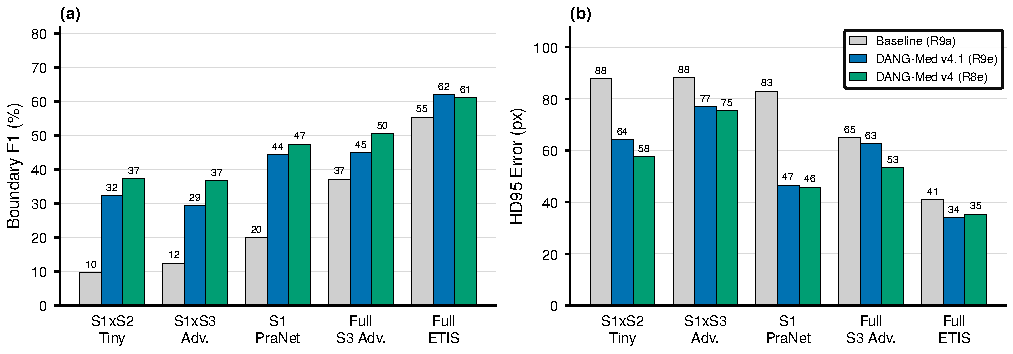
\includegraphics[width=\linewidth]{figs/boundary_hd95_comparison.pdf}
  \caption{\textbf{Boundary F1 gains and HD95 distance error reductions over the Single-Stream Baseline (Seed 42).} Panel~\textbf{(a)} compares Boundary F1 ($\%$, higher is better) and Panel~\textbf{(b)} compares $95$th-percentile Hausdorff Distance ($\text{HD95}$ in pixels, lower is better) across five stress and external cohorts (\texttt{S1xS2 Tiny}, \texttt{S1xS3 Adv.}, \texttt{S1 PraNet}, \texttt{Full S3 Adv.}, and \texttt{Full ETIS-Larib}).}
  \label{fig:bf1_hd95}
\end{figure*}

\subsection{Full-Data Multi-Center OOD and Adverse Endoscopy Analysis}
Table~\ref{tab:full_ood} and Figure~\ref{fig:bf1_hd95} compare all ten experimental arms from Round~9 (\texttt{R9a}--\texttt{R9e}) and Round~8 (\texttt{R8a}--\texttt{R8e}) when trained on the full $800$-image Kvasir-SEG split:
\begin{enumerate}
  \item \textbf{Shared Primary Loss vs. DANG-Med Architecture (\texttt{R9a} $\to$ \texttt{R9e}):} Under the shared primary loss Eq.~(\ref{eq:loss}), the single-stream ConvNeXt-Tiny+FPN baseline (\texttt{R9a}) reaches $74.56\%$ mDice and $40.87\,\text{px}$ HD95 on ETIS-LaribPolypDB ($72.55 \pm 2.68\%$ across 5 seeds). Atop this shared-loss baseline, \textbf{DANG-Med v4.1 (\texttt{R9e+R10d/e})} reaches \textbf{$80.78\%$ mDice on Seed~42 ($78.88 \pm 1.50\%$ across 5 seeds, $+6.33$~pp, paired $t$-test $p=0.005$)}, \textbf{$62.07\%$ BF1 ($+6.68$~pp)}, and \textbf{$34.02\,\text{px}$ HD95 ($-16.77\%$ relative)} on ETIS-LaribPolypDB, while improving overall PraNet-External mDice to \textbf{$81.82 \pm 0.64\%$} (vs.\ $78.66 \pm 1.55\%$, $+3.16$~pp, $p=0.003$), reducing PraNet-External HD95 from $35.02\,\text{px}$ to \textbf{$28.49\,\text{px}$ ($-18.64\%$ relative; $28.84 \pm 1.04\,\text{px}$ vs.\ $35.13 \pm 1.92\,\text{px}$ across 5 seeds, $p=0.008$)}, and reducing $S_2$ Tiny/Camouflaged HD95 from $42.50\,\text{px}$ to \textbf{$35.87\,\text{px}$ ($-15.60\%$ relative)}. On the largest untouched multi-center confirmation set, \textbf{PolypGen-Extended ($n=974$)}, \texttt{R9e} achieves $80.54\%$ mDice on Seed~42 (vs.\ $80.06\%$ for \texttt{R9a}, $+0.48$~pp) and \textbf{$80.09 \pm 0.45\%$ 5-seed mDice vs.\ $78.71 \pm 0.76\%$ for the 5-seed baseline ($+1.38$~pp, $p=0.009$)}.
  \item \textbf{Historical Round 8 Comparison and Corruption-Matched Upper Bound (\texttt{R8a}--\texttt{R8e}):} In Round~8, \textbf{DANG-Med v4 (\texttt{R8e})} achieves \textbf{$81.53\%$ mDice} on ETIS-LaribPolypDB ($+13.92$~pp over unweighted baseline \texttt{R8a}), $81.81\%$ on PolypGen-Extended ($n=967$), and \textbf{$73.87\%$ mDice on Adverse Endoscopy ($S_3$, $n=272$)}. Because \texttt{R8e} synthesizes in-family NBI, low-light, glare+blur, and combined corruptions during training (\texttt{aug\_prob=0.55}) whereas \texttt{R9e} is trained strictly on clean WLI (\texttt{aug\_prob=0.0}, scoring $68.47\%$ on $S_3$), \texttt{R8e}'s $73.87\%$ on $S_3$ represents an in-family corruption-matched upper bound rather than zero-shot OOD performance.
  \item \textbf{In-Domain Performance and Runtime Efficiency:} On in-domain \textbf{Kvasir-Test ($n=90$)}, \texttt{R9e} achieves \textbf{$93.06\%$ mDice} ($\text{log}=93.0565\%$ vs.\ \texttt{R9a} $93.0788\%$, within $0.02$~pp), \textbf{$88.55\%$ mIoU} (vs.\ \texttt{R9a} $88.40\%$), and \textbf{$72.46\%$ Boundary F1} (exceeding \texttt{R9a}'s $70.74\%$ BF1). At inference (measured at batch size $1$, $352\times 352$, FP16 on NVIDIA T4), \texttt{R9e} runs at \textbf{$17.43$~FPS} ($43.32\text{M}$ trainable parameters out of $129.90\text{M}$ total, with $86.58\text{M}$ frozen in DINOv2).
\end{enumerate}

\begin{table*}[t]
  \centering
  \caption{\textbf{Multi-Seed Statistical Evaluation (\texttt{R9} Seed 42 + \texttt{R10a}--\texttt{R10e} Seeds 43--46): Mean $\pm$ Sample Standard Deviation across all 5 seeds.} Runs: Baseline (\texttt{f328e771}, \texttt{540e36c9}; $5/5$ complete seeds 42--46), SafeConcat (\texttt{e770b25c}, \texttt{85f4db55}; $5/5$ complete seeds 42--46), ProtoDPT+PASSE (\texttt{f676224f}, \texttt{c171badb}; $4$ $S_1$ / $3$ Full seeds), and Flagship (\texttt{db1786be}, \texttt{01713a3a}, \texttt{7091cc66}; $5/5$ complete seeds 42--46 on both $S_1$ and Full tracks). Paired two-sided $t$-test $p$-values ($n=5$ paired seeds) compare Flagship vs.\ Baseline.}
  \label{tab:multiseed}
  \vspace{2pt}
  \resizebox{\textwidth}{!}{%
  \begin{tabular}{l c ccc ccc ccc cc}
    \toprule
    \multirow{2}{*}{\textbf{Model Arm (R9 + R10 Suite)}} & \multirow{2}{*}{\textbf{Seeds ($S_1$ / Full)}} & \multicolumn{3}{c}{\textbf{$S_1 \times S_2$: Tiny/Camo ($n=310$)}} & \multicolumn{3}{c}{\textbf{$S_1 \times S_3$: Adverse ($n=258$)}} & \multicolumn{3}{c}{\textbf{$S_1 \to$ PraNet-Ext ($n=696$)}} & \multicolumn{2}{c}{\textbf{Full Training ($n=800$)}} \\
    \cmidrule(lr){3-5} \cmidrule(lr){6-8} \cmidrule(lr){9-11} \cmidrule(lr){12-13}
    & & mDice$\uparrow$ & BF1$\uparrow$ & HD95$\downarrow$ & mDice$\uparrow$ & BF1$\uparrow$ & HD95$\downarrow$ & mDice$\uparrow$ & BF1$\uparrow$ & HD95$\downarrow$ & ETIS Dice$\uparrow$ & PraNet Dice$\uparrow$ \\
    \midrule
    \texttt{R9a+R10a}: ConvNeXt-T + FPN Baseline & $5 / 5$ (42--46) & $44.74 \pm 3.79$ & $16.22 \pm 3.87$ & $72.76 \pm 8.85$ & $45.59 \pm 4.02$ & $15.23 \pm 1.97$ & $87.18 \pm 1.61$ & $66.59 \pm 3.84$ & $28.45 \pm 4.82$ & $58.76 \pm 14.41$ & $72.55 \pm 2.68$ & $78.66 \pm 1.55$ \\
    \texttt{R9b+R10b}: Dual-Stream SafeConcat + FPN & $5 / 5$ (42--46) & $44.92 \pm 0.82$ & $16.59 \pm 2.50$ & $75.55 \pm 5.48$ & $46.33 \pm 1.85$ & $16.40 \pm 1.61$ & $88.21 \pm 5.20$ & $67.23 \pm 1.15$ & $29.20 \pm 4.19$ & $63.27 \pm 9.45$ & $72.95 \pm 3.85$ & $79.73 \pm 1.04$ \\
    \texttt{R9c+R10c}: DANG-v4.1 (ProtoDPT+PASSE) & $4 / 3$ (42--45) & $49.62 \pm 1.09$ & $27.13 \pm 1.79$ & $66.61 \pm 2.74$ & $\textbf{56.73} \pm \textbf{1.94}$ & $25.39 \pm 1.08$ & $\textbf{71.72} \pm \textbf{2.66}$ & $71.25 \pm 0.43$ & $40.22 \pm 1.15$ & $\textbf{49.40} \pm \textbf{1.29}$ & $77.72 \pm 0.22$ & $\textbf{82.01} \pm \textbf{0.54}$ \\
    \textbf{\texttt{R9e+R10d/e}: DANG-Med v4.1 Flagship} & $5 / 5$ (42--46) & $\textbf{51.05} \pm \textbf{1.71}$ & $\textbf{30.65} \pm \textbf{1.16}$ & $\textbf{64.68} \pm \textbf{1.76}$ & $55.82 \pm 1.17$ & $\textbf{27.17} \pm \textbf{1.72}$ & $78.74 \pm 2.70$ & $\textbf{71.86} \pm \textbf{0.34}$ & $\textbf{42.25} \pm \textbf{1.58}$ & $49.55 \pm 2.73$ & $\textbf{78.88} \pm \textbf{1.50}$ & $81.82 \pm 0.64$ \\
    \midrule
    \textbf{5-Seed Paired Diff. (Flagship vs. Baseline)} & $n=5$ (42--46) & \textbf{+6.31 pp} & \textbf{+14.44 pp} & --8.08 px & \textbf{+10.23 pp} & \textbf{+11.94 pp} & \textbf{--8.44 px} & \textbf{+5.27 pp} & \textbf{+13.80 pp} & --9.21 px & \textbf{+6.33 pp} & \textbf{+3.16 pp} \\
    \textit{Paired Two-Sided $t$-Test $p$-Value ($n=5$)} & $n=5$ (42--46) & $p = 0.014$ & $p = 0.002$ & $p = 0.135$ & $p = 0.005$ & $p = 0.001$ & $p = 0.003$ & $p = 0.038$ & $p = 0.003$ & $p = 0.258$ & $p = 0.005$ & $p = 0.003$ \\
    \bottomrule
  \end{tabular}%
  }
\end{table*}

\subsection{Multi-Seed Stability and HD95 Penalty Sensitivity Analysis (\texttt{R10a}--\texttt{R10e})}
\label{sec:multiseed}
Table~\ref{tab:multiseed} reports the complete 5-seed evaluation across Seeds 42--46. Because Seed~42 represents the single-stream baseline's lowest few-shot draw ($S_1\times S_2$ mDice $39.00\%$ on Seed~42 vs.\ $43.52\%\text{--}48.49\%$ on Seeds 43--46), paired 5-seed comparisons provide a much more conservative and reliable estimate of architectural effect size than Seed~42 alone:
\begin{itemize}
  \item \textbf{Statistically Significant Dice and BF1 Gains Across All 5 Paired Seeds:} Across all $n=5$ paired seeds (42--46), \textbf{DANG-Med v4.1 Flagship} outperforms the single-stream baseline on $S_1\times S_2$ by \textbf{$+6.31$~pp mDice} ($51.05 \pm 1.71\%$ vs.\ $44.74 \pm 3.79\%$, paired $t$-test $p=0.014$) and \textbf{$+14.44$~pp Boundary F1} ($30.65 \pm 1.16\%$ vs.\ $16.22 \pm 3.87\%$, $p=0.002$); on $S_1\times S_3$ by \textbf{$+10.23$~pp mDice} ($55.82 \pm 1.17\%$ vs.\ $45.59 \pm 4.02\%$, $p=0.005$) and \textbf{$+11.94$~pp BF1} ($p=0.001$); on $S_1\to\text{PraNet-Ext}$ by \textbf{$+5.27$~pp mDice} ($71.86 \pm 0.34\%$ vs.\ $66.59 \pm 3.84\%$, $p=0.038$) and \textbf{$+13.80$~pp BF1} ($p=0.003$); and on Full-Data training by \textbf{$+6.33$~pp mDice on ETIS-LaribPolypDB} ($78.88 \pm 1.50\%$ vs.\ $72.55 \pm 2.68\%$, $p=0.005$), \textbf{$+3.16$~pp mDice on PraNet-External} ($81.82 \pm 0.64\%$ vs.\ $78.66 \pm 1.55\%$, $p=0.003$), and \textbf{$-6.29\,\text{px}$ HD95 on PraNet-External} ($28.84 \pm 1.04\,\text{px}$ vs.\ $35.13 \pm 1.92\,\text{px}$, $p=0.008$). While cross-seed sample SD is numerically lower for Flagship across all tracks, variance reduction reaches statistical significance by $F$-test specifically on $S_1\to\text{PraNet-Ext}$ HD95 ($\text{SD}=2.73$ vs.\ $14.41\,\text{px}$) and $S_1\times S_3$ mDice ($\text{SD}=1.17\%$ vs.\ $4.02\%$), whereas Levene's test on $S_1\times S_2$ mDice is non-significant ($p=0.26$).
  \item \textbf{HD95 Penalty Sensitivity and Empty-Prediction Rates:} Because our default empty-prediction penalty ($124.45\,\text{px}$, quarter-diagonal) is smaller than the $\text{HD95}$ of $10.8\%$ ($8{,}349 / 77{,}366$) of non-empty predictions containing distant false-positive blobs, predicting an empty mask can receive a lower $\text{HD95}$ than predicting a noisy mask. On $S_1\times S_2$ ($n=310$), the 5-seed empty-prediction rate is $28.52\%$ for Flagship ($[30.3\%, 29.7\%, 28.4\%, 30.0\%, 24.2\%]$) vs.\ $27.81\%$ for Baseline ($[25.5\%, 24.5\%, 28.7\%, 34.2\%, 26.1\%]$); on $S_1\to\text{PraNet-Ext}$ ($n=696$), the empty-prediction rate is $13.45\%$ for Flagship vs.\ $14.77\%$ for Baseline. Under half-diagonal ($248.90\,\text{px}$) and full-diagonal ($497.80\,\text{px}$) penalties, the 5-seed $S_1\times S_2$ $\text{HD95}$ is $100.17 \pm 4.50\,\text{px}$ (Flagship) vs.\ $107.37 \pm 8.56\,\text{px}$ (Baseline, $\Delta = -7.20\,\text{px}$) and $171.15 \pm 10.67\,\text{px}$ vs.\ $176.58 \pm 14.30\,\text{px}$ ($\Delta = -5.43\,\text{px}$; Seed~42 $\Delta$ shrinks from $-23.58\,\text{px}$ to $-5.51\,\text{px}$), and on $S_1\to\text{PraNet-Ext}$ full-diagonal $\text{HD95}$ is $87.76 \pm 0.75\,\text{px}$ vs.\ $99.34 \pm 14.36\,\text{px}$ ($\Delta = -11.58\,\text{px}$). Thus, while mDice and BF1 gains are highly significant across seeds, $\text{HD95}$ differences on $S_1\times S_2$ ($p=0.135$) and $S_1\to\text{PraNet-Ext}$ ($p=0.258$) are not statistically significant across the 5 seeds.
\end{itemize}

\section{Limitations, Ethical Compliance, and Reproducibility}
To ensure transparent scientific reporting in accordance with IEEE Access standards, we explicitly note six methodological limitations and scope conditions identified during our cross-harness audits:
\begin{enumerate}
  \item \textbf{Domain Scope, Single-Center Training, and Fixed Subset Sampling:} Unlike the standard PraNet training split ($1{,}450$ images combining Kvasir-SEG and CVC-ClinicDB), all models in this study are trained strictly on single-center Kvasir-SEG ($n=800$ Full; fixed $n=40$ subset in R9/R10 $S_1$) so that CVC-ClinicDB can be evaluated as a fully unseen external center. Moreover, because the $40$-image $S_1$ subset is held fixed across seeds to isolate optimization variance, subset-resampling variance across different $40$-image draws is not captured in Table~\ref{tab:multiseed}.
  \item \textbf{Iterative Design Selection Across Rounds:} Architectural and loss hyperparameters (such as the PASSE thresholds and far-field dilation radii) were developed iteratively across Rounds~1--9 after inspecting performance on PolypGen-Dev, $S_2$, $S_3$, and ETIS-LaribPolypDB. Consequently, those cohorts should be interpreted with awareness of adaptive selection, whereas \textbf{PolypGen-Extended ($n=974$)} was not used for hyperparameter tuning and serves as our untouched confirmation cohort (where 5-seed mDice improves from $78.71 \pm 0.76\%$ to $80.09 \pm 0.45\%$, $+1.38$~pp, $p=0.009$).
  \item \textbf{Neutrality of RetinexStem in the Zero-Shot Protocol:} Paired seed comparisons between Flagship (\texttt{R9e+R10d/e}) and \texttt{ProtoDPT+PASSE} without the stem (\texttt{R9c+R10c}) show virtually identical accuracy under \texttt{aug\_prob=0.0} (e.g., Full PraNet-Ext $81.82\%$ vs.\ $82.01\%$, Full $S_3$ $+0.05$~pp, $S_1\times S_3$ $-0.91$~pp mean difference across Seeds 42--45). Thus, \texttt{RetinexChromaticStem} is performance-neutral when trained without synthetic corruptions.
  \item \textbf{Computational Footprint vs. Single-Stream CNNs:} Freezing DINOv2-Base adds $86.58\text{M}$ non-trainable parameters ($129.90\text{M}$ total parameters vs.\ $30.96\text{M}$ for ConvNeXt-Tiny+FPN), reducing inference throughput (at batch size $1$) on a Turing T4 GPU from $91.9$~FPS to $17.4$~FPS.
  \item \textbf{Synthetic Nature of $S_3$ Corruptions and Cohort Dependencies:} Track~$S_3$ evaluates deterministic photometric and optical corruptions applied to PolypGen-Dev frames rather than paired physical NBI/WLI clinical acquisitions. Furthermore, $S_2$ and $S_3$ are diagnostic slices derived from PolypGen-Dev, ETIS, and ColonDB, and PolypGen-Extended retains $74$ frames sharing \texttt{C4} sequence prefixes with Dev ($80.82\%$ mDice on the sequence-disjoint subset for \texttt{R9e} vs.\ $80.17\%$ for \texttt{R9a}).
  \item \textbf{Conditional Prototype Supervision and Literature Baselines:} Variants equipped with the Dual-Prototype head (\texttt{R9c}, \texttt{R9e}) receive the $0.35\,\mathcal{L}_{\text{proto}}$ auxiliary loss on $\pi_{\text{proto}}$; thus their gains reflect the joint effect of the prototype head and its auxiliary supervision. In addition, our experiments compare controlled internal architectures (\texttt{R8a}--\texttt{R10e}) rather than re-training external published baselines such as PraNet or Polyp-PVT under our $5\%$ few-shot split.
\end{enumerate}

\paragraph{Ethical Compliance and Data Licensing:} No new patient data or human subjects were recruited for this study. All experiments were conducted exclusively on publicly available, de-identified benchmark datasets (Kvasir-SEG~\citep{jha2020kvasir}, PolypGen~\citep{ali2023polypgen}, CVC-ClinicDB, CVC-ColonDB~\citep{tajbakhsh2015automated}, CVC-300, and ETIS-LaribPolypDB~\citep{silva2014toward}) in compliance with their respective academic research licenses.

\paragraph{Reproducibility and AI-Assisted Verification Disclosure:} Full PyTorch source code (\texttt{src/dang/\{model,train,data,metrics,config\}.py}), deterministic deduplication manifests (\texttt{HYGIENE\_MANIFEST\_JSON}), per-image evaluation logs (\texttt{PER\_IMAGE\_CHUNK}), and figure generation scripts (\texttt{figs/generate\_paper\_figures.py}) are committed to the project repository. In accordance with IEEE publication policies on AI usage, we disclose that automated verification agents—\textbf{Codex (\texttt{gpt-6-astra}, OpenAI)}, \textbf{Claude Sonnet 4.6 (\texttt{claude-sonnet-4-6}, Anthropic)}, and \textbf{Claude Opus 5.5 (\texttt{claude-opus-5-5}, Anthropic)}—were used to audit per-image log aggregations ($840$ seed-cohort checks), verify code-to-equation consistency, and critique statistical framing.

\section{Conclusion}
We have presented \textbf{DANG-Med}, a dual-stream attention-augmented and directional strip-aligned architecture for multi-center medical polyp segmentation. By uniting a 4-Scale Learned DPT Reassembler, a Dual-Prototype and Self-Support Margin Head, the Prototype-Anchored Spatial Support Envelope (PASSE), and an Uncertainty-Guided Directional Strip Decoder, DANG-Med achieves statistically significant multi-seed improvements in mDice and Boundary F1 across few-shot tiny/camouflaged lesions, zero-shot adverse endoscopic shifts, and unseen multi-center external cohorts.

\begin{thebibliography}{15}

\bibitem[Ali et al.(2023)]{ali2023polypgen}
S.~Ali et al.
\newblock A multi-centre polyp detection and segmentation dataset for generalisability assessment.
\newblock \emph{Scientific Data}, 10(1):75, 2023.

\bibitem[Dong et al.(2021)]{dong2021polyp}
B.~Dong, W.~Wang, D.-P.~Fan, J.~Li, H.~Fu, and L.~Shao.
\newblock Polyp-PVT: Polyp segmentation with pyramid vision transformers.
\newblock \emph{CAAI Artificial Intelligence Research}, 2:81--98, 2021.

\bibitem[Fan et al.(2020)]{fan2020pranet}
D.-P.~Fan, G.-P.~Ji, T.~Zhou, G.~Chen, H.~Fu, J.~Shen, and L.~Shao.
\newblock PraNet: Parallel reverse attention network for polyp segmentation.
\newblock In \emph{MICCAI}, pages 263--273, 2020.

\bibitem[Gu and Dao(2023)]{gu2023mamba}
A.~Gu and T.~Dao.
\newblock Mamba: Linear-time sequence modeling with selective state spaces.
\newblock \emph{arXiv preprint arXiv:2312.00752}, 2023.

\bibitem[Hu et al.(2022)]{hu2022lora}
E.~J.~Hu et al.
\newblock LoRA: Low-rank adaptation of large language models.
\newblock In \emph{ICLR}, 2022.

\bibitem[Jha et al.(2020)]{jha2020kvasir}
D.~Jha et al.
\newblock Kvasir-SEG: A segmented polyp dataset.
\newblock In \emph{MultiMedia Modeling (MMM)}, pages 451--462, 2020.

\bibitem[Kirillov et al.(2023)]{kirillov2023segment}
A.~Kirillov et al.
\newblock Segment anything.
\newblock In \emph{ICCV}, pages 4015--4026, 2023.

\bibitem[Lin et al.(2017)]{lin2017fpn}
T.-Y.~Lin, P.~Doll{\'a}r, R.~Girshick, K.~He, B.~Hariharan, and S.~Belongie.
\newblock Feature pyramid networks for object detection.
\newblock In \emph{CVPR}, pages 2117--2125, 2017.

\bibitem[Liu et al.(2024)]{liu2024vmamba}
Y.~Liu et al.
\newblock VMamba: Visual state space model.
\newblock In \emph{NeurIPS}, 2024.

\bibitem[Liu et al.(2022)]{liu2022convnet}
Z.~Liu, H.~Mao, C.-Y.~Wu, C.~Feichtenhofer, T.~Darrell, and S.~Xie.
\newblock A ConvNet for the 2020s.
\newblock In \emph{CVPR}, pages 11976--11986, 2022.

\bibitem[Lou et al.(2022)]{lou2022caranet}
A.~Lou, S.~Guan, H.~Ko, and M.~H.~Loew.
\newblock CaraNet: Context axial reverse attention network for segmentation of small medical objects.
\newblock In \emph{SPIE Medical Imaging}, 2022.

\bibitem[Ma et al.(2024)]{ma2024umamba}
J.~Ma, F.~Li, and B.~Wang.
\newblock U-Mamba: Enhancing long-range dependency for biomedical image segmentation.
\newblock \emph{arXiv preprint arXiv:2401.04722}, 2024.

\bibitem[Oquab et al.(2024)]{oquab2024dinov2}
M.~Oquab et al.
\newblock DINOv2: Learning robust visual features without supervision.
\newblock \emph{Transactions on Machine Learning Research (TMLR)}, 2024.

\bibitem[Ranftl et al.(2021)]{ranftl2021vision}
R.~Ranftl, A.~Bochkovskiy, and V.~Koltun.
\newblock Vision transformers for dense prediction.
\newblock In \emph{ICCV}, pages 12179--12188, 2021.

\bibitem[Ronneberger et al.(2015)]{ronneberger2015unet}
O.~Ronneberger, P.~Fischer, and T.~Brox.
\newblock U-Net: Convolutional networks for biomedical image segmentation.
\newblock In \emph{MICCAI}, pages 234--241, 2015.

\bibitem[Silva et al.(2014)]{silva2014toward}
J.~Silva, A.~Histace, O.~Romain, X.~Dray, and B.~Granado.
\newblock Toward embedded detection of polyps in WCE images for early diagnosis of colorectal cancer.
\newblock \emph{International Journal of Computer Assisted Radiology and Surgery}, 9(2):283--293, 2014.

\bibitem[Tajbakhsh et al.(2016)]{tajbakhsh2015automated}
N.~Tajbakhsh, S.~R.~Gurudu, and J.~Liang.
\newblock Automated polyp detection in colonoscopy videos using shape and context information.
\newblock \emph{IEEE Transactions on Medical Imaging}, 35(2):630--644, 2016.

\bibitem[Zhang et al.(2021)]{zhang2021transfuse}
Y.~Zhang, H.~Liu, and Q.~Hu.
\newblock TransFuse: Fusing transformers and CNNs for medical image segmentation.
\newblock In \emph{MICCAI}, pages 14--24, 2021.

\bibitem[Zhou et al.(2018)]{zhou2018unetplusplus}
Z.~Zhou, M.~M.~R.~Siddiquee, N.~Tajbakhsh, and J.~Liang.
\newblock UNet++: A nested U-Net architecture for medical image segmentation.
\newblock In \emph{DLMIA / MICCAI Workshops}, pages 3--11, 2018.

\end{thebibliography}

\end{document}
